\documentclass[border=15pt]{standalone}
\usepackage{amsmath, amssymb}
\usepackage{tikz}
\usetikzlibrary{arrows.meta}

\definecolor{block0}{HTML}{E53935}
\definecolor{block1}{HTML}{1E88E5}

\begin{document}
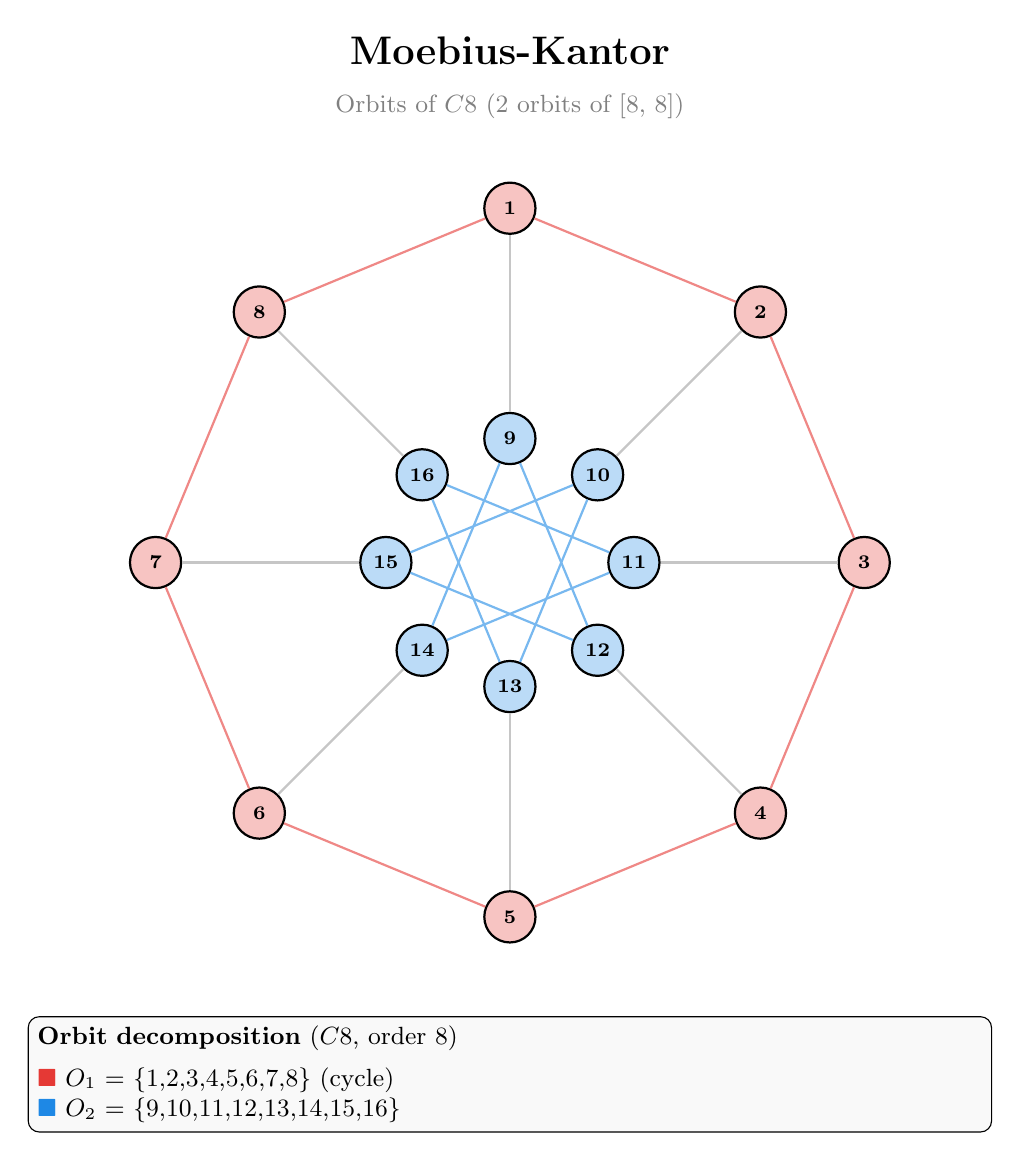
\begin{tikzpicture}[
  vertex/.style={circle, draw, thick, minimum size=6.5mm, inner sep=0pt,
                 font=\scriptsize\bfseries},
  edge/.style={thick, gray!45},
  title/.style={font=\Large\bfseries},
  subtitle/.style={font=\small, text=gray},
]

\node[title] at (0, 6.5) {Moebius-Kantor};
\node[subtitle] at (0, 5.8) {Orbits of $C8$ (2 orbits of [8, 8])};

\node[vertex, fill=block0!30] (v1) at (0.000, 4.500) {1};
\node[vertex, fill=block0!30] (v2) at (3.182, 3.182) {2};
\node[vertex, fill=block0!30] (v3) at (4.500, -0.000) {3};
\node[vertex, fill=block0!30] (v4) at (3.182, -3.182) {4};
\node[vertex, fill=block0!30] (v5) at (-0.000, -4.500) {5};
\node[vertex, fill=block0!30] (v6) at (-3.182, -3.182) {6};
\node[vertex, fill=block0!30] (v7) at (-4.500, 0.000) {7};
\node[vertex, fill=block0!30] (v8) at (-3.182, 3.182) {8};
\node[vertex, fill=block1!30] (v9) at (0.000, 1.575) {9};
\node[vertex, fill=block1!30] (v10) at (1.114, 1.114) {10};
\node[vertex, fill=block1!30] (v11) at (1.575, -0.000) {11};
\node[vertex, fill=block1!30] (v12) at (1.114, -1.114) {12};
\node[vertex, fill=block1!30] (v13) at (-0.000, -1.575) {13};
\node[vertex, fill=block1!30] (v14) at (-1.114, -1.114) {14};
\node[vertex, fill=block1!30] (v15) at (-1.575, 0.000) {15};
\node[vertex, fill=block1!30] (v16) at (-1.114, 1.114) {16};

\draw[thick, block0!60] (v1) -- (v2);
\draw[thick, block0!60] (v1) -- (v8);
\draw[edge] (v1) -- (v9);
\draw[thick, block0!60] (v2) -- (v3);
\draw[edge] (v2) -- (v10);
\draw[thick, block0!60] (v3) -- (v4);
\draw[edge] (v3) -- (v11);
\draw[thick, block0!60] (v4) -- (v5);
\draw[edge] (v4) -- (v12);
\draw[thick, block0!60] (v5) -- (v6);
\draw[edge] (v5) -- (v13);
\draw[thick, block0!60] (v6) -- (v7);
\draw[edge] (v6) -- (v14);
\draw[thick, block0!60] (v7) -- (v8);
\draw[edge] (v7) -- (v15);
\draw[edge] (v8) -- (v16);
\draw[thick, block1!60] (v9) -- (v12);
\draw[thick, block1!60] (v9) -- (v14);
\draw[thick, block1!60] (v10) -- (v13);
\draw[thick, block1!60] (v10) -- (v15);
\draw[thick, block1!60] (v11) -- (v14);
\draw[thick, block1!60] (v11) -- (v16);
\draw[thick, block1!60] (v12) -- (v15);
\draw[thick, block1!60] (v13) -- (v16);

\node[draw, rounded corners, fill=gray!5, text width=12cm, align=left, font=\small]
  at (0, -6.5) {
  \textbf{Orbit decomposition} ($C8$, order 8) \\[4pt]
  \textcolor{block0}{$\blacksquare$} $O_{1}$ = \{1,2,3,4,5,6,7,8\} (cycle) \\
  \textcolor{block1}{$\blacksquare$} $O_{2}$ = \{9,10,11,12,13,14,15,16\}
};

\end{tikzpicture}
\end{document}